The expected number of signal and background events for an integrated 
luminosity of 1\ifb{} after applying the 
\WW\ like selection are reported in Tab.~\ref{tab:wwselection0}(0-jet), Tab.~\ref{tab:wwselection1}(1-jet), Tab.~\ref{tab:wwselection2}(VBF).
The corresponding $\Delta\phi$, di-lepton mass, di-lepton $p_T$, $m_T$ and projected $\met$ distributions are shown in Figs.~\ref{fig:dPhi_jets0}-\ref{fig:pmet_jets0}(0-jet)
and Figs.~\ref{fig:dPhi_jets1}-\ref{fig:pmet_jets1}(1-jet).

\begin{table}[!ht]
  \begin{center}
 {\small
  \begin{tabular} {|c|c|c|c|c|c|c|c|c|c|c|}
\hline
  & DY(ee) & DY($\mu\mu$) & DY($\tau\tau$) & ttbar & TW & Wjets & WZ & ZZ & ggWW & qqWW \\
  \hline
  \hline
  mm &  0.0$\pm$0.0 &  2.5$\pm$1.5 &  0.0$\pm$0.0 &  7.0$\pm$1.0 &  3.2$\pm$0.3 &  8.7$\pm$4.4 &  3.1$\pm$0.2 &  2.3$\pm$0.1 &  4.5$\pm$0.1 & 77.5$\pm$0.7 \\
  me &  0.0$\pm$0.0 &  0.8$\pm$0.8 &  0.0$\pm$0.0 & 11.2$\pm$1.3 &  4.1$\pm$0.3 & 34.9$\pm$8.7 &  2.6$\pm$0.2 &  0.2$\pm$0.0 &  5.0$\pm$0.1 & 102.4$\pm$0.8 \\
  em &  0.0$\pm$0.0 &  0.0$\pm$0.0 &  0.0$\pm$0.0 & 11.0$\pm$1.3 &  4.7$\pm$0.3 & 42.9$\pm$9.6 &  3.6$\pm$0.2 &  0.3$\pm$0.0 &  5.8$\pm$0.1 & 121.2$\pm$0.9 \\
  ee &  0.8$\pm$0.8 &  0.0$\pm$0.0 &  0.8$\pm$0.8 &  3.8$\pm$0.8 &  2.2$\pm$0.2 & 24.7$\pm$7.1 &  1.6$\pm$0.1 &  1.2$\pm$0.1 &  2.8$\pm$0.1 & 46.7$\pm$0.5 \\
 \hline
 all &  0.8$\pm$0.8 &  3.4$\pm$1.7 &  0.8$\pm$0.8 & 33.0$\pm$2.2 & 14.3$\pm$0.6 & 111.1$\pm$15.4 & 10.9$\pm$0.3 &  3.9$\pm$0.1 & 18.2$\pm$0.2 & 347.8$\pm$1.5 \\
 \hline
  \end{tabular}
  }
 {\small
  \begin{tabular} {|c|c|c|c|c|c|c|c|c|c|c|}
  \hline
     &   H$_{120}$ &  H$_{130}$ &    H$_{140}$ &   H$_{150}$ &   H$_{160}$ &   H$_{170}$ &   H$_{180}$ &   H$_{190}$ &   H$_{200}$ &   H$_{250}$ \\
  \hline
  \hline
  mm &  3.5$\pm$0.1 &  8.0$\pm$0.1 & 13.5$\pm$0.2 & 18.6$\pm$0.2 & 24.2$\pm$0.3 & 22.5$\pm$0.3 & 16.9$\pm$0.2 & 10.9$\pm$0.1 &  8.4$\pm$0.1 &  4.2$\pm$0.1 \\
  me &  2.7$\pm$0.1 &  6.7$\pm$0.1 & 11.7$\pm$0.2 & 16.4$\pm$0.2 & 22.0$\pm$0.3 & 20.0$\pm$0.3 & 16.7$\pm$0.2 & 12.5$\pm$0.2 & 10.1$\pm$0.1 &  5.5$\pm$0.1 \\
  em &  4.4$\pm$0.1 &  9.5$\pm$0.1 & 15.2$\pm$0.2 & 19.4$\pm$0.2 & 23.7$\pm$0.3 & 22.8$\pm$0.3 & 18.8$\pm$0.2 & 13.9$\pm$0.2 & 11.4$\pm$0.1 &  6.3$\pm$0.1 \\
  ee &  1.6$\pm$0.0 &  4.0$\pm$0.1 &  7.6$\pm$0.1 & 11.2$\pm$0.2 & 15.3$\pm$0.2 & 14.7$\pm$0.2 & 11.5$\pm$0.2 &  7.2$\pm$0.1 &  5.8$\pm$0.1 &  2.8$\pm$0.1 \\
  \hline
 all & 12.2$\pm$0.1 & 28.3$\pm$0.2 & 48.0$\pm$0.4 & 65.5$\pm$0.5 & 85.2$\pm$0.6 & 79.9$\pm$0.5 & 63.8$\pm$0.4 & 44.6$\pm$0.3 & 35.7$\pm$0.2 & 18.7$\pm$0.1 \\
 \hline
  \end{tabular}
  }
  \caption{Expected number of signal and background events for an 
  integrated luminosity of 1\ifb{} after 
  applying the \ww\ 0-jet selection requirements. Monte Carlo statistical uncertainties are 
  included.}
   \label{tab:wwselection0}
  \end{center}
\end{table}

\begin{table}[!ht]
  \begin{center}
 {\small
  \begin{tabular} {|c|c|c|c|c|c|c|c|c|c|c|}
\hline
  & DY(ee) & DY($\mu\mu$) & DY($\tau\tau$) & ttbar & TW & Wjets & WZ & ZZ & ggWW & qqWW \\
  \hline
  \hline
  mm &  0.0$\pm$0.0 & 27.7$\pm$4.8 &  0.0$\pm$0.0 & 73.7$\pm$3.3 & 19.1$\pm$0.6 &  2.2$\pm$2.2 &  1.6$\pm$0.1 &  0.7$\pm$0.0 &  1.4$\pm$0.0 & 25.2$\pm$0.4 \\
  me &  0.0$\pm$0.0 &  0.8$\pm$0.8 &  0.0$\pm$0.0 & 100.8$\pm$3.9 & 23.5$\pm$0.7 &  8.7$\pm$4.4 &  2.3$\pm$0.1 &  0.1$\pm$0.0 &  1.7$\pm$0.0 & 32.2$\pm$0.4 \\
  em &  0.0$\pm$0.0 &  2.5$\pm$1.5 &  5.0$\pm$2.0 & 108.6$\pm$4.0 & 28.8$\pm$0.8 &  6.4$\pm$3.7 &  3.5$\pm$0.2 &  0.2$\pm$0.0 &  2.2$\pm$0.1 & 38.0$\pm$0.5 \\
  ee & 16.2$\pm$3.6 &  0.0$\pm$0.0 &  0.0$\pm$0.0 & 45.6$\pm$2.6 & 12.1$\pm$0.5 &  4.1$\pm$2.9 &  1.6$\pm$0.1 &  0.4$\pm$0.0 &  0.9$\pm$0.0 & 15.1$\pm$0.3 \\
 \hline
 all & 16.2$\pm$3.6 & 31.1$\pm$5.1 &  5.0$\pm$2.0 & 328.7$\pm$7.0 & 83.4$\pm$1.3 & 21.4$\pm$6.8 &  8.9$\pm$0.3 &  1.5$\pm$0.1 &  6.3$\pm$0.1 & 110.6$\pm$0.8 \\
 \hline
  \end{tabular}
  }
 {\small
  \begin{tabular} {|c|c|c|c|c|c|c|c|c|c|c|}
  \hline
     &   H$_{120}$ &  H$_{130}$ &    H$_{140}$ &   H$_{150}$ &   H$_{160}$ &   H$_{170}$ &   H$_{180}$ &   H$_{190}$ &   H$_{200}$ &   H$_{250}$ \\
  \hline
  \hline
  mm &  1.4$\pm$0.0 &  3.2$\pm$0.1 &  5.9$\pm$0.1 &  8.4$\pm$0.2 & 11.9$\pm$0.2 & 11.4$\pm$0.2 &  9.5$\pm$0.2 &  6.3$\pm$0.1 &  4.8$\pm$0.1 &  2.6$\pm$0.1 \\
  me &  1.3$\pm$0.0 &  3.2$\pm$0.1 &  6.0$\pm$0.1 &  8.4$\pm$0.2 & 11.6$\pm$0.2 & 11.0$\pm$0.2 &  9.7$\pm$0.2 &  7.0$\pm$0.1 &  6.0$\pm$0.1 &  3.7$\pm$0.1 \\
  em &  1.9$\pm$0.0 &  4.3$\pm$0.1 &  7.2$\pm$0.1 & 10.0$\pm$0.2 & 12.7$\pm$0.2 & 12.6$\pm$0.2 & 10.7$\pm$0.2 &  8.2$\pm$0.1 &  6.8$\pm$0.1 &  4.3$\pm$0.1 \\
  ee &  0.7$\pm$0.0 &  1.9$\pm$0.1 &  3.4$\pm$0.1 &  5.3$\pm$0.1 &  7.9$\pm$0.2 &  7.6$\pm$0.2 &  6.1$\pm$0.1 &  4.0$\pm$0.1 &  3.2$\pm$0.1 &  1.9$\pm$0.0 \\
  \hline
  all &  5.4$\pm$0.1 & 12.6$\pm$0.2 & 22.5$\pm$0.2 & 32.1$\pm$0.3 & 44.1$\pm$0.4 & 42.6$\pm$0.4 & 35.9$\pm$0.3 & 25.4$\pm$0.2 & 20.9$\pm$0.2 & 12.5$\pm$0.1 \\

 \hline
  \end{tabular}
  }
 {\small
  \begin{tabular} {|c|c|c|c|c|c|c|c|c|c|c|}
  \hline
     &   H$^{VBF}_{120}$ &  H$^{VBF}_{130}$ &    H$^{VBF}_{140}$ &   H$^{VBF}_{150}$ &   H$^{VBF}_{160}$ &   H$^{VBF}_{170}$ &   H$^{VBF}_{180}$ &   H$^{VBF}_{190}$ &   H$^{VBF}_{200}$ &   H$^{VBF}_{250}$ \\
  \hline
  \hline
  mm &  0.1$\pm$0.0 &  0.4$\pm$0.0 &  0.7$\pm$0.0 &  1.0$\pm$0.0 &  1.5$\pm$0.0 &  1.5$\pm$0.0 &  1.2$\pm$0.0 &  0.9$\pm$0.0 &  0.7$\pm$0.0 &  0.4$\pm$0.0 \\
  me &  0.1$\pm$0.0 &  0.4$\pm$0.0 &  0.7$\pm$0.0 &  1.0$\pm$0.0 &  1.4$\pm$0.0 &  1.5$\pm$0.0 &  1.3$\pm$0.0 &  1.0$\pm$0.0 &  0.9$\pm$0.0 &  0.6$\pm$0.0 \\
  em &  0.2$\pm$0.0 &  0.5$\pm$0.0 &  0.8$\pm$0.0 &  1.2$\pm$0.0 &  1.6$\pm$0.0 &  1.6$\pm$0.0 &  1.5$\pm$0.0 &  1.2$\pm$0.0 &  1.0$\pm$0.0 &  0.6$\pm$0.0 \\
  ee &  0.1$\pm$0.0 &  0.2$\pm$0.0 &  0.4$\pm$0.0 &  0.6$\pm$0.0 &  0.9$\pm$0.0 &  1.0$\pm$0.0 &  0.8$\pm$0.0 &  0.6$\pm$0.0 &  0.5$\pm$0.0 &  0.3$\pm$0.0 \\
  \hline
 all &  0.6$\pm$0.0 &  1.4$\pm$0.0 &  2.5$\pm$0.0 &  3.8$\pm$0.0 &  5.3$\pm$0.0 &  5.6$\pm$0.0 &  4.8$\pm$0.0 &  3.7$\pm$0.0 &  3.1$\pm$0.0 &  1.8$\pm$0.0 \\


 \hline
  \end{tabular}
  }
  \caption{Expected number of signal and background events for an 
  integrated luminosity of 1\ifb{} after 
  applying the \ww\ 1-jet selection requirements. Monte Carlo statistical uncertainties are 
  included.}
   \label{tab:wwselection1}
  \end{center}
\end{table}



\begin{table}[!ht]
  \begin{center}
 {\small
  \begin{tabular} {|c|c|c|c|c|c|c|c|c|c|c|}
\hline
  & DY(ee) & DY($\mu\mu$) & DY($\tau\tau$) & ttbar & TW & Wjets & WZ & ZZ & ggWW & qqWW \\
  \hline
  \hline
  mm &  0.0$\pm$0.0 &  5.9$\pm$2.2 &  0.0$\pm$0.0 & 31.2$\pm$2.1 &  2.8$\pm$0.2 &  0.0$\pm$0.0 &  0.1$\pm$0.0 &  0.1$\pm$0.0 &  0.1$\pm$0.0 &  1.6$\pm$0.1 \\
  me &  0.0$\pm$0.0 &  0.0$\pm$0.0 &  0.0$\pm$0.0 & 43.2$\pm$2.5 &  4.0$\pm$0.3 &  2.2$\pm$2.2 &  0.2$\pm$0.0 &  0.0$\pm$0.0 &  0.2$\pm$0.0 &  2.1$\pm$0.1 \\
  em &  0.0$\pm$0.0 &  0.0$\pm$0.0 &  0.0$\pm$0.0 & 51.4$\pm$2.8 &  5.0$\pm$0.3 &  4.4$\pm$3.1 &  0.3$\pm$0.1 &  0.0$\pm$0.0 &  0.2$\pm$0.0 &  2.6$\pm$0.1 \\
  ee &  1.6$\pm$1.1 &  0.0$\pm$0.0 &  0.0$\pm$0.0 & 21.5$\pm$1.8 &  2.6$\pm$0.2 &  0.0$\pm$0.0 &  0.2$\pm$0.0 &  0.0$\pm$0.0 &  0.1$\pm$0.0 &  1.0$\pm$0.1 \\
 \hline
 all &  1.6$\pm$1.1 &  5.9$\pm$2.2 &  0.0$\pm$0.0 & 147.3$\pm$4.7 & 14.3$\pm$0.6 &  6.5$\pm$3.8 &  0.8$\pm$0.1 &  0.1$\pm$0.0 &  0.6$\pm$0.0 &  7.4$\pm$0.2 \\

 \hline
  \end{tabular}
  }
 {\small
  \begin{tabular} {|c|c|c|c|c|c|c|c|c|c|c|}
  \hline
     &   H$_{120}$ &  H$_{130}$ &    H$_{140}$ &   H$_{150}$ &   H$_{160}$ &   H$_{170}$ &   H$_{180}$ &   H$_{190}$ &   H$_{200}$ &   H$_{250}$ \\
  \hline
  \hline
  mm &  0.1$\pm$0.0 &  0.3$\pm$0.0 &  0.6$\pm$0.0 &  0.8$\pm$0.1 &  1.3$\pm$0.1 &  1.2$\pm$0.1 &  1.1$\pm$0.1 &  0.7$\pm$0.0 &  0.5$\pm$0.0 &  0.3$\pm$0.0 \\
  me &  0.1$\pm$0.0 &  0.3$\pm$0.0 &  0.6$\pm$0.0 &  0.9$\pm$0.1 &  1.1$\pm$0.1 &  1.2$\pm$0.1 &  1.1$\pm$0.1 &  0.9$\pm$0.0 &  0.7$\pm$0.0 &  0.5$\pm$0.0 \\
  em &  0.2$\pm$0.0 &  0.4$\pm$0.0 &  0.8$\pm$0.0 &  1.0$\pm$0.1 &  1.4$\pm$0.1 &  1.3$\pm$0.1 &  1.4$\pm$0.1 &  1.0$\pm$0.0 &  0.9$\pm$0.0 &  0.5$\pm$0.0 \\
  ee &  0.1$\pm$0.0 &  0.2$\pm$0.0 &  0.4$\pm$0.0 &  0.5$\pm$0.0 &  0.8$\pm$0.1 &  0.8$\pm$0.1 &  0.6$\pm$0.0 &  0.4$\pm$0.0 &  0.4$\pm$0.0 &  0.2$\pm$0.0 \\
  \hline
 all &  0.5$\pm$0.0 &  1.3$\pm$0.0 &  2.4$\pm$0.1 &  3.3$\pm$0.1 &  4.6$\pm$0.1 &  4.5$\pm$0.1 &  4.2$\pm$0.1 &  3.0$\pm$0.1 &  2.4$\pm$0.1 &  1.5$\pm$0.0 \\
 \hline
  \end{tabular}
  }
 {\small
  \begin{tabular} {|c|c|c|c|c|c|c|c|c|c|c|}
  \hline
     &   H$^{VBF}_{120}$ &  H$^{VBF}_{130}$ &    H$^{VBF}_{140}$ &   H$^{VBF}_{150}$ &   H$^{VBF}_{160}$ &   H$^{VBF}_{170}$ &   H$^{VBF}_{180}$ &   H$^{VBF}_{190}$ &   H$^{VBF}_{200}$ &   H$^{VBF}_{250}$ \\
  \hline
  \hline
  mm &  0.1$\pm$0.0 &  0.4$\pm$0.0 &  0.6$\pm$0.0 &  1.0$\pm$0.0 &  1.4$\pm$0.0 &  1.5$\pm$0.0 &  1.3$\pm$0.0 &  0.9$\pm$0.0 &  0.7$\pm$0.0 &  0.4$\pm$0.0 \\
  me &  0.2$\pm$0.0 &  0.4$\pm$0.0 &  0.7$\pm$0.0 &  1.0$\pm$0.0 &  1.5$\pm$0.0 &  1.5$\pm$0.0 &  1.3$\pm$0.0 &  1.1$\pm$0.0 &  1.0$\pm$0.0 &  0.6$\pm$0.0 \\
  em &  0.2$\pm$0.0 &  0.5$\pm$0.0 &  0.9$\pm$0.0 &  1.2$\pm$0.0 &  1.6$\pm$0.0 &  1.7$\pm$0.0 &  1.6$\pm$0.0 &  1.3$\pm$0.0 &  1.1$\pm$0.0 &  0.7$\pm$0.0 \\
  ee &  0.1$\pm$0.0 &  0.2$\pm$0.0 &  0.4$\pm$0.0 &  0.6$\pm$0.0 &  0.9$\pm$0.0 &  1.0$\pm$0.0 &  0.8$\pm$0.0 &  0.6$\pm$0.0 &  0.5$\pm$0.0 &  0.3$\pm$0.0 \\
  \hline
 all &  0.6$\pm$0.0 &  1.4$\pm$0.0 &  2.6$\pm$0.0 &  3.8$\pm$0.0 &  5.5$\pm$0.0 &  5.7$\pm$0.0 &  5.0$\pm$0.0 &  3.8$\pm$0.0 &  3.2$\pm$0.0 &  2.0$\pm$0.0 \\

 \hline
  \end{tabular}
  }
  \caption{Expected number of signal and background events for an 
  integrated luminosity of 1\ifb{} after 
  applying the \ww\ selection requirements, requiring only 2-jets in the event with $|\Delta\eta|>2.0$.
  Monte Carlo statistical uncertainties are  included.}
   \label{tab:wwselection2}
  \end{center}
\end{table}


\begin{figure}[!hbtp]
\centering
\subfigure[]{
\centering
\label{subfig:dPhi_hm120_jets0}
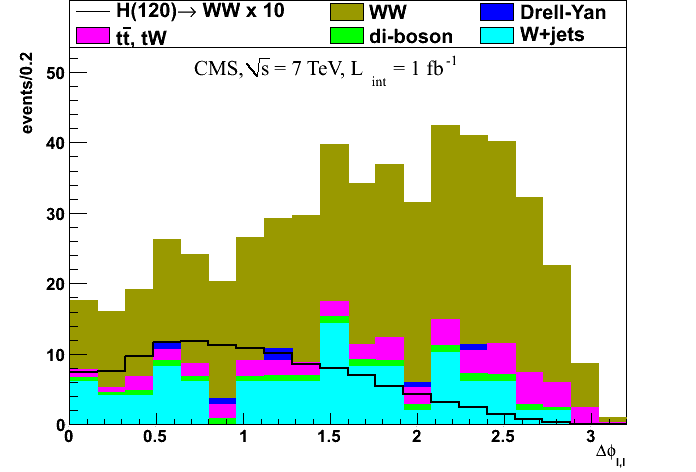
\includegraphics[width=.32\textwidth]{figures/dPhi_hm120_jets0.png}}
\subfigure[]{
\centering
\label{subfig:dPhi_hm160_jets0}
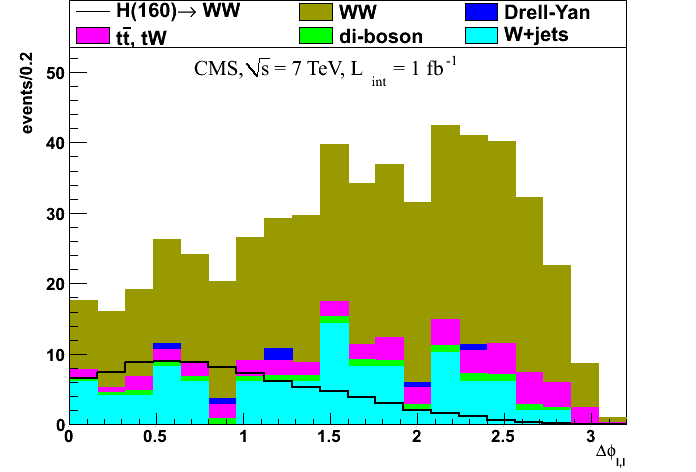
\includegraphics[width=.32\textwidth]{figures/dPhi_hm160_jets0.png}}
\subfigure[]{
\centering
\label{subfig:dPhi_hm250_jets0}
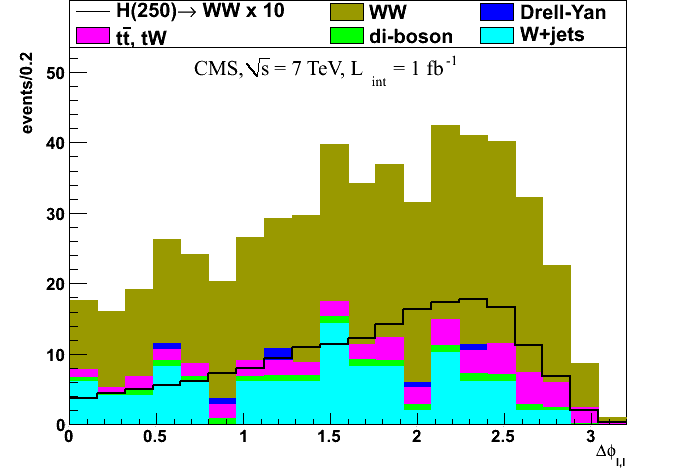
\includegraphics[width=.32\textwidth]{figures/dPhi_hm250_jets0.png}}\\
\caption{Lepton $\Delta\phi$ distribution after \WW\ selection for $m_H$=120 $\GeVcc$ \subref{subfig:dPhi_hm120_jets0}, 
$m_H$=160 $\GeVcc$ \subref{subfig:dPhi_hm160_jets0} and $m_H$=250 $\GeVcc$ \subref{subfig:dPhi_hm250_jets0} in the 0-jet bin.}
\label{fig:dPhi_jets0}
\end{figure}

\begin{figure}[!hbtp]
\centering
\subfigure[]{
\centering
\label{subfig:dilepmass_hm120_jets0}
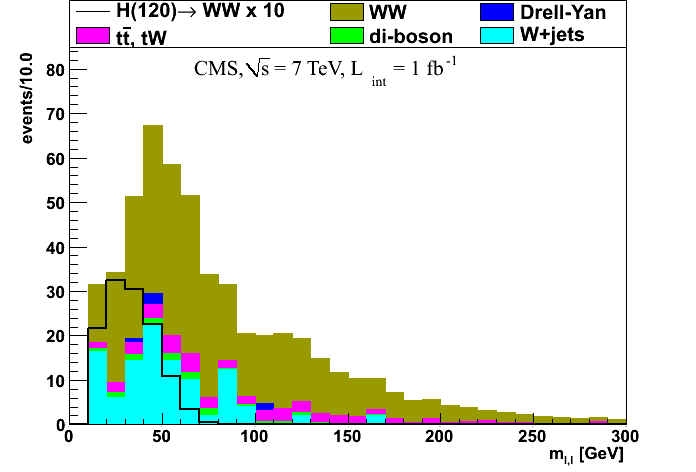
\includegraphics[width=.32\textwidth]{figures/dilepmass_hm120_jets0.png}}
\subfigure[]{
\centering
\label{subfig:dilepmass_hm160_jets0}
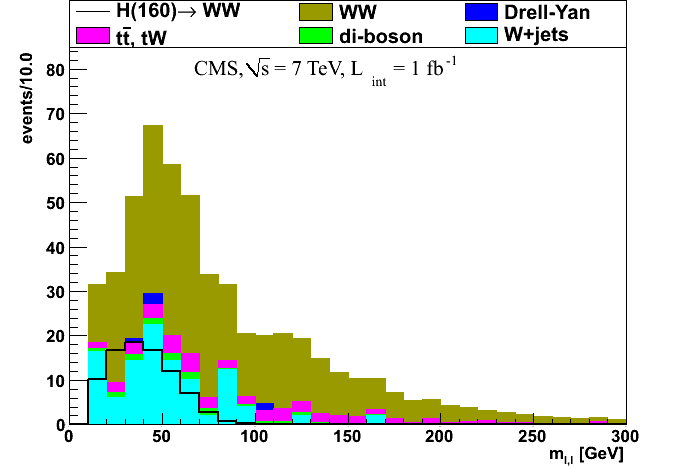
\includegraphics[width=.32\textwidth]{figures/dilepmass_hm160_jets0.png}}
\subfigure[]{
\centering
\label{subfig:dilepmass_hm250_jets0}
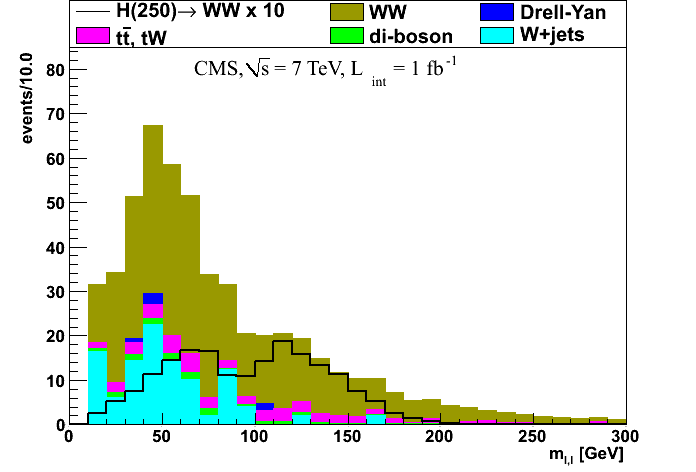
\includegraphics[width=.32\textwidth]{figures/dilepmass_hm250_jets0.png}}\\
\caption{Di-lepton mass distribution after \WW\ selection for $m_H$=120 $\GeVcc$ \subref{subfig:dilepmass_hm120_jets0}, 
$m_H$=160 $\GeVcc$ \subref{subfig:dilepmass_hm160_jets0} and $m_H$=250 $\GeVcc$ \subref{subfig:dilepmass_hm250_jets0} in the 0-jet bin.}
\label{fig:dilepmass_jets0}
\end{figure}

\begin{figure}[!hbtp]
\centering
\subfigure[]{
\centering
\label{subfig:dileppt_hm120_jets0}
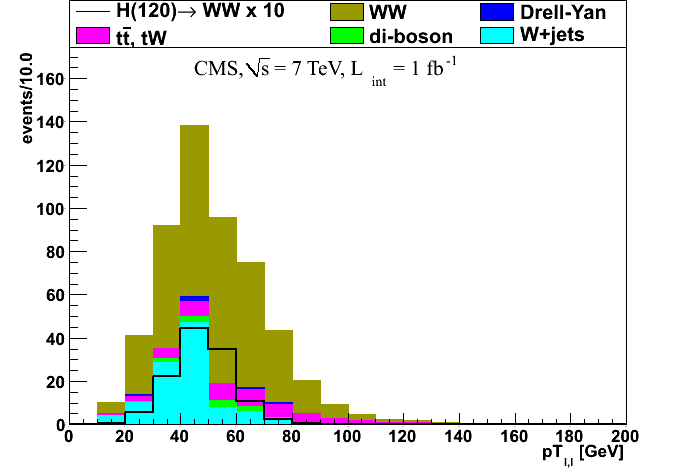
\includegraphics[width=.32\textwidth]{figures/dileppt_hm120_jets0.png}}
\subfigure[]{
\centering
\label{subfig:dileppt_hm160_jets0}
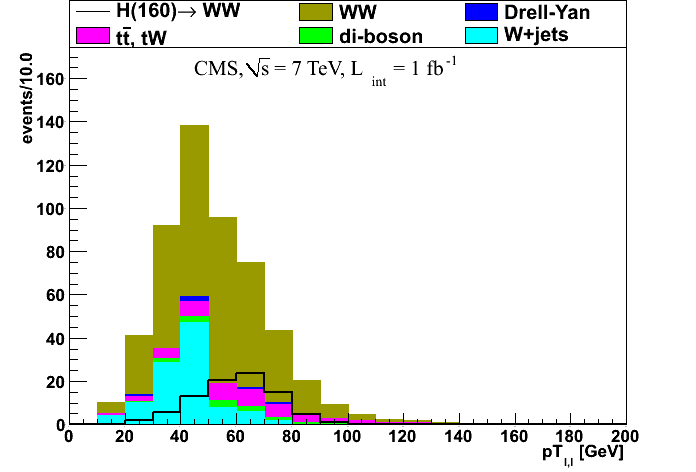
\includegraphics[width=.32\textwidth]{figures/dileppt_hm160_jets0.png}}
\subfigure[]{
\centering
\label{subfig:dileppt_hm250_jets0}
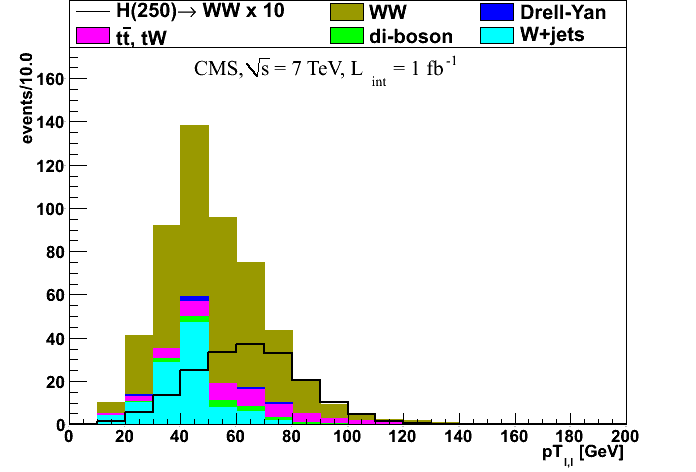
\includegraphics[width=.32\textwidth]{figures/dileppt_hm250_jets0.png}}\\
\caption{Di-lepton $p_T$ distribution after \WW\ selection for $m_H$=120 $\GeVcc$ \subref{subfig:dileppt_hm120_jets0}, 
$m_H$=160 $\GeVcc$ \subref{subfig:dileppt_hm160_jets0} and $m_H$=250 $\GeVcc$ \subref{subfig:dileppt_hm250_jets0} in the 0-jet bin.}
\label{fig:dileppt_jets0}
\end{figure}

\begin{figure}[!hbtp]
\centering
\subfigure[]{
\centering
\label{subfig:mt_hm120_jets0}
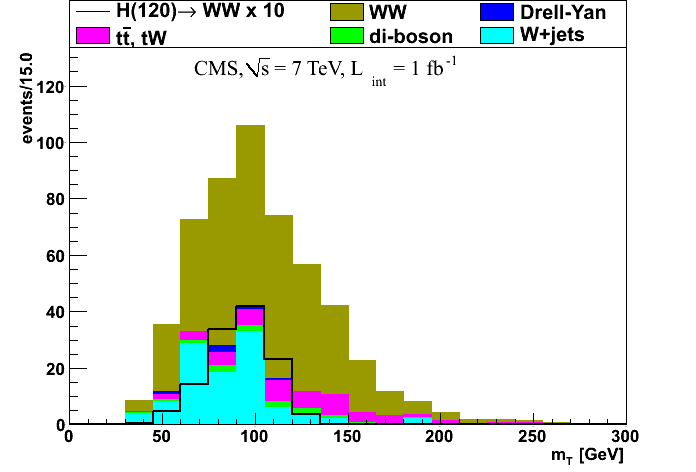
\includegraphics[width=.32\textwidth]{figures/mt_hm120_jets0.png}}
\subfigure[]{
\centering
\label{subfig:mt_hm160_jets0}
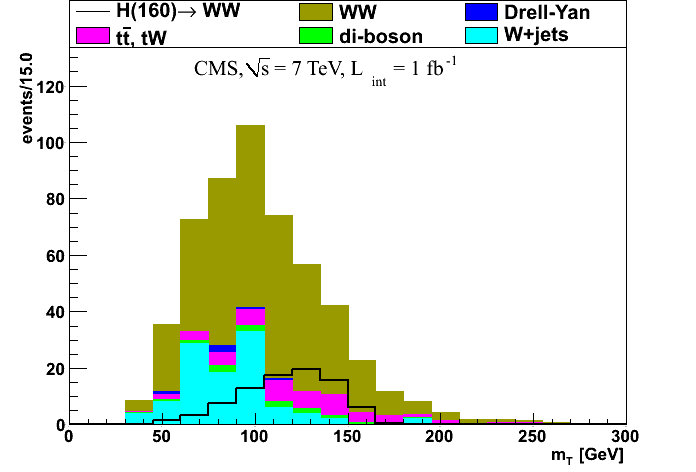
\includegraphics[width=.32\textwidth]{figures/mt_hm160_jets0.png}}
\subfigure[]{
\centering
\label{subfig:mt_hm250_jets0}
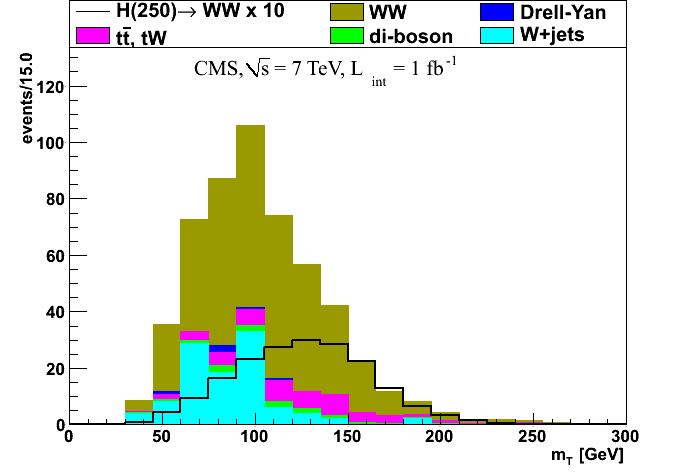
\includegraphics[width=.32\textwidth]{figures/mt_hm250_jets0.png}}\\
\caption{$m_T$ distribution after \WW\ selection for $m_H$=120 $\GeVcc$ \subref{subfig:mt_hm120_jets0}, 
$m_H$=160 $\GeVcc$ \subref{subfig:mt_hm160_jets0} and $m_H$=250 $\GeVcc$ \subref{subfig:mt_hm250_jets0} in the 0-jet bin.}
\label{fig:mt_jets0}
\end{figure}

\begin{figure}[!hbtp]
\centering
\subfigure[]{
\centering
\label{subfig:pmet_hm120_jets0}
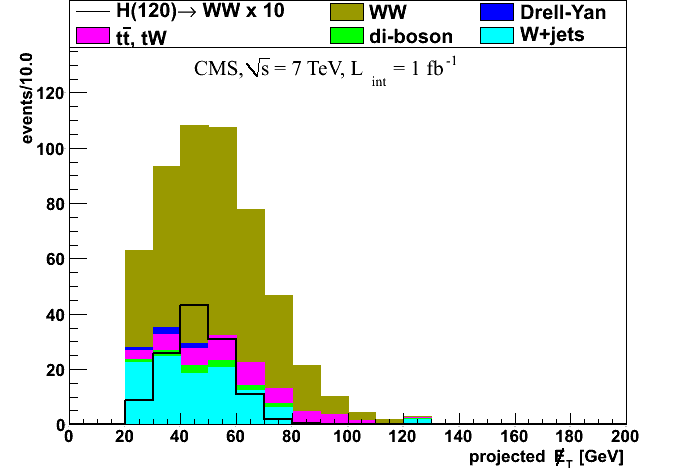
\includegraphics[width=.32\textwidth]{figures/pmet_hm120_jets0.png}}
\subfigure[]{
\centering
\label{subfig:pmet_hm160_jets0}
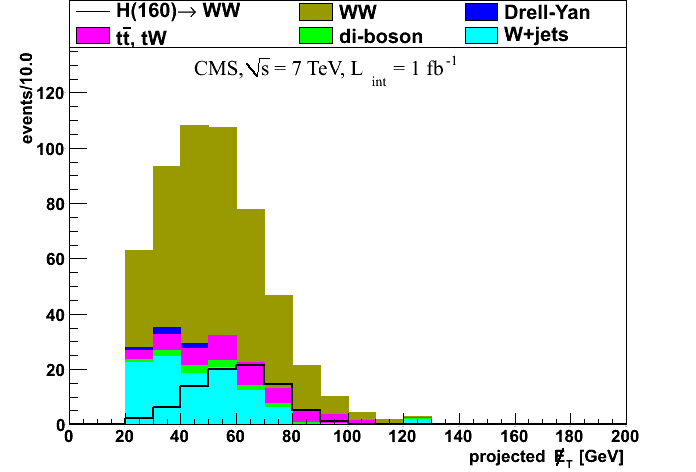
\includegraphics[width=.32\textwidth]{figures/pmet_hm160_jets0.png}}
\subfigure[]{
\centering
\label{subfig:pmet_hm250_jets0}
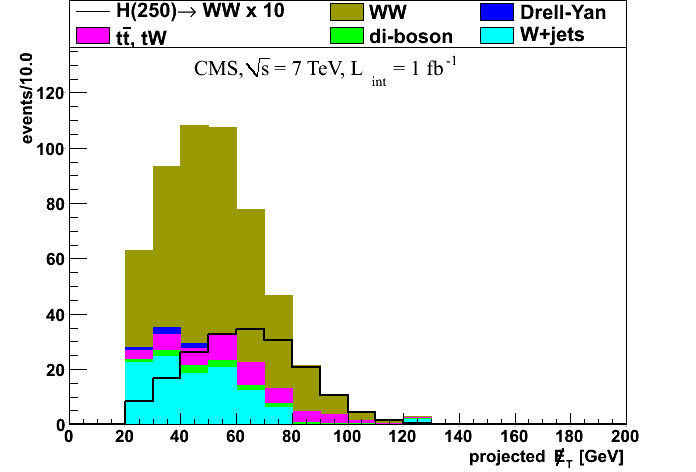
\includegraphics[width=.32\textwidth]{figures/pmet_hm250_jets0.png}}\\
\caption{Projected $\met$ distribution after \WW\ selection for $m_H$=120 $\GeVcc$ \subref{subfig:pmet_hm120_jets0}, 
$m_H$=160 $\GeVcc$ \subref{subfig:pmet_hm160_jets0} and $m_H$=250 $\GeVcc$ \subref{subfig:pmet_hm250_jets0} in the 0-jet bin.}
\label{fig:pmet_jets0}
\end{figure}








\begin{figure}[!hbtp]
\centering
\subfigure[]{
\centering
\label{subfig:dPhi_hm120_jets1}
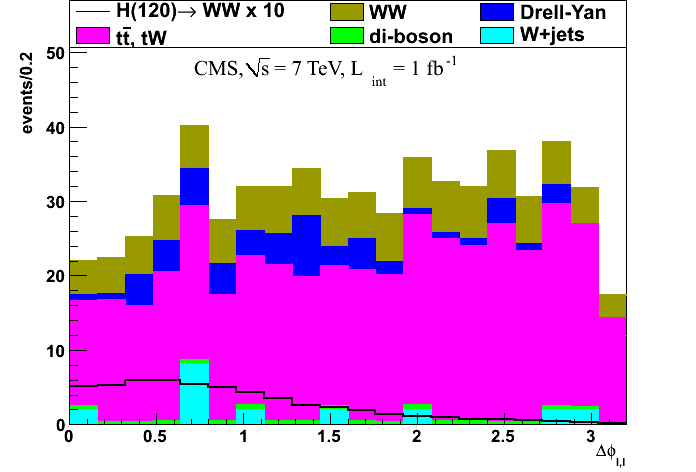
\includegraphics[width=.32\textwidth]{figures/dPhi_hm120_jets1.png}}
\subfigure[]{
\centering
\label{subfig:dPhi_hm160_jets1}
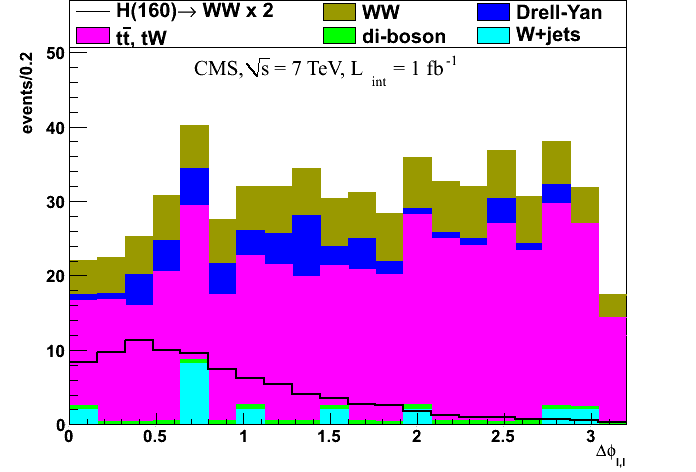
\includegraphics[width=.32\textwidth]{figures/dPhi_hm160_jets1.png}}
\subfigure[]{
\centering
\label{subfig:dPhi_hm250_jets1}
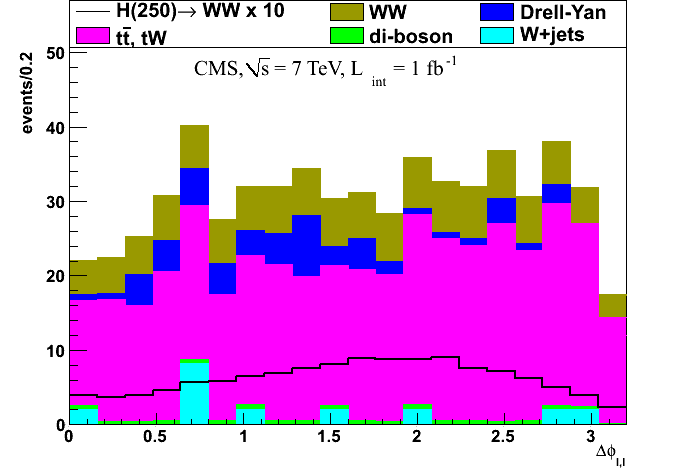
\includegraphics[width=.32\textwidth]{figures/dPhi_hm250_jets1.png}}\\
\caption{Lepton $\Delta\phi$ distribution after \WW\ selection for $m_H$=120 $\GeVcc$ \subref{subfig:dPhi_hm120_jets1}, 
$m_H$=160 $\GeVcc$ \subref{subfig:dPhi_hm160_jets1} and $m_H$=250 $\GeVcc$ \subref{subfig:dPhi_hm250_jets1} in the 1-jet bin.}
\label{fig:dPhi_jets1}
\end{figure}

\begin{figure}[!hbtp]
\centering
\subfigure[]{
\centering
\label{subfig:dilepmass_hm120_jets1}
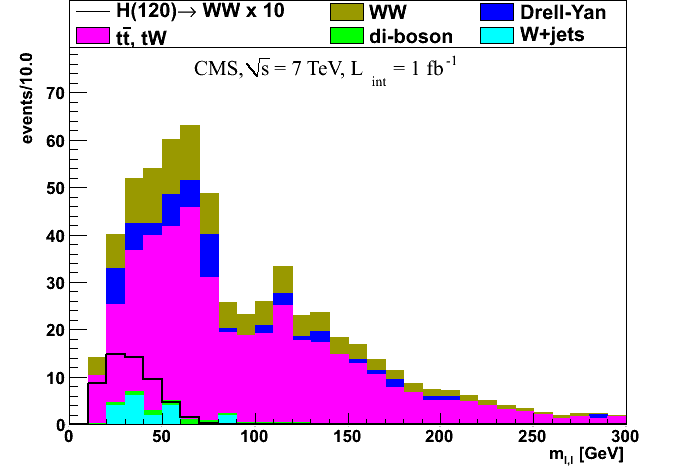
\includegraphics[width=.32\textwidth]{figures/dilepmass_hm120_jets1.png}}
\subfigure[]{
\centering
\label{subfig:dilepmass_hm160_jets1}
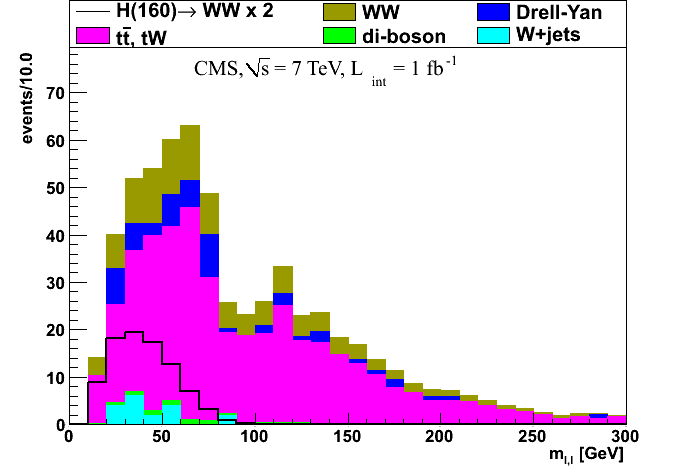
\includegraphics[width=.32\textwidth]{figures/dilepmass_hm160_jets1.png}}
\subfigure[]{
\centering
\label{subfig:dilepmass_hm250_jets1}
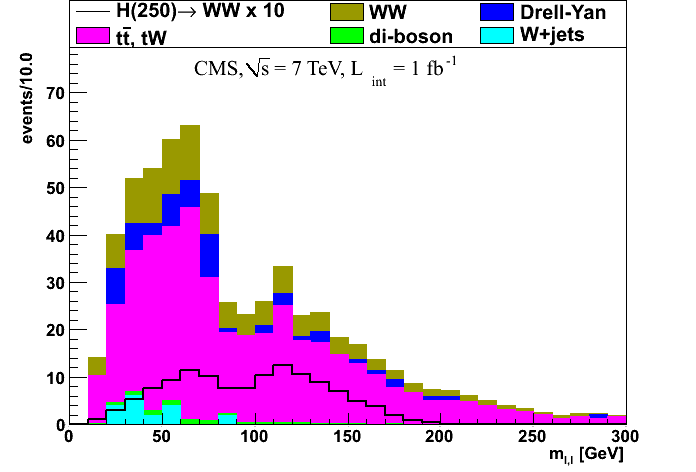
\includegraphics[width=.32\textwidth]{figures/dilepmass_hm250_jets1.png}}\\
\caption{Di-lepton mass distribution after \WW\ selection for $m_H$=120 $\GeVcc$ \subref{subfig:dilepmass_hm120_jets1}, 
$m_H$=160 $\GeVcc$ \subref{subfig:dilepmass_hm160_jets1} and $m_H$=250 $\GeVcc$ \subref{subfig:dilepmass_hm250_jets1} in the 1-jet bin.}
\label{fig:dilepmass_jets1}
\end{figure}

\begin{figure}[!hbtp]
\centering
\subfigure[]{
\centering
\label{subfig:dileppt_hm120_jets1}
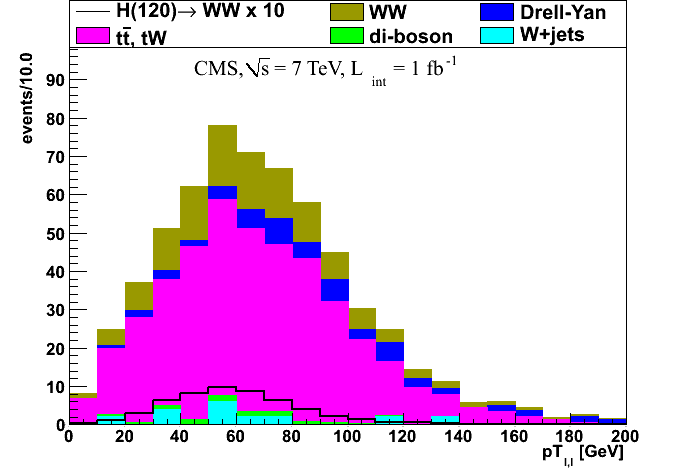
\includegraphics[width=.32\textwidth]{figures/dileppt_hm120_jets1.png}}
\subfigure[]{
\centering
\label{subfig:dileppt_hm160_jets1}
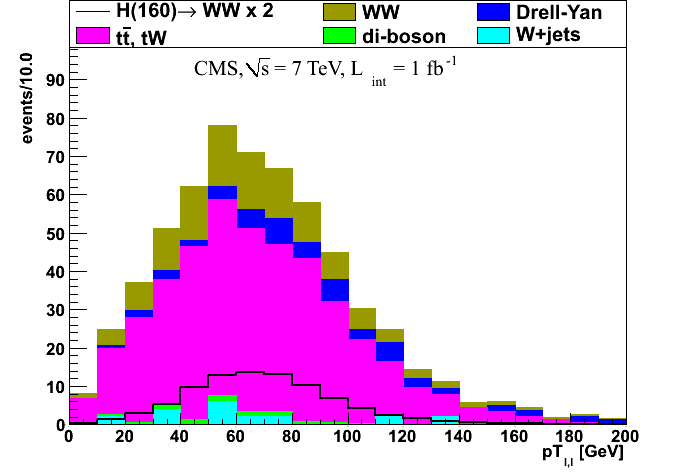
\includegraphics[width=.32\textwidth]{figures/dileppt_hm160_jets1.png}}
\subfigure[]{
\centering
\label{subfig:dileppt_hm250_jets1}
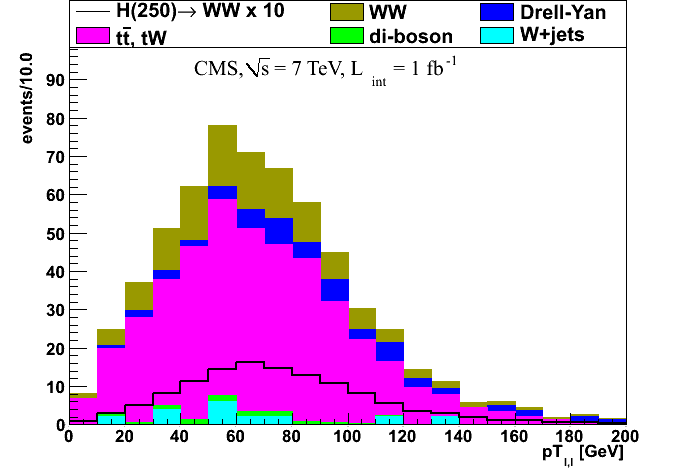
\includegraphics[width=.32\textwidth]{figures/dileppt_hm250_jets1.png}}\\
\caption{Di-lepton $p_T$ distribution after \WW\ selection for $m_H$=120 $\GeVcc$ \subref{subfig:dileppt_hm120_jets1}, 
$m_H$=160 $\GeVcc$ \subref{subfig:dileppt_hm160_jets1} and $m_H$=250 $\GeVcc$ \subref{subfig:dileppt_hm250_jets1} in the 1-jet bin.}
\label{fig:dileppt_jets1}
\end{figure}

\begin{figure}[!hbtp]
\centering
\subfigure[]{
\centering
\label{subfig:mt_hm120_jets1}
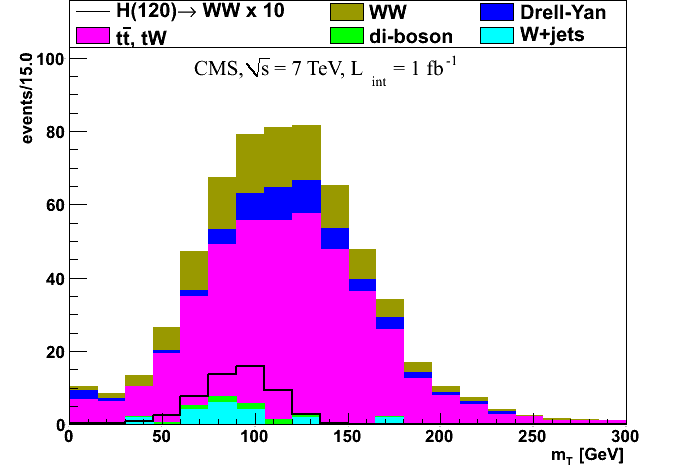
\includegraphics[width=.32\textwidth]{figures/mt_hm120_jets1.png}}
\subfigure[]{
\centering
\label{subfig:mt_hm160_jets1}
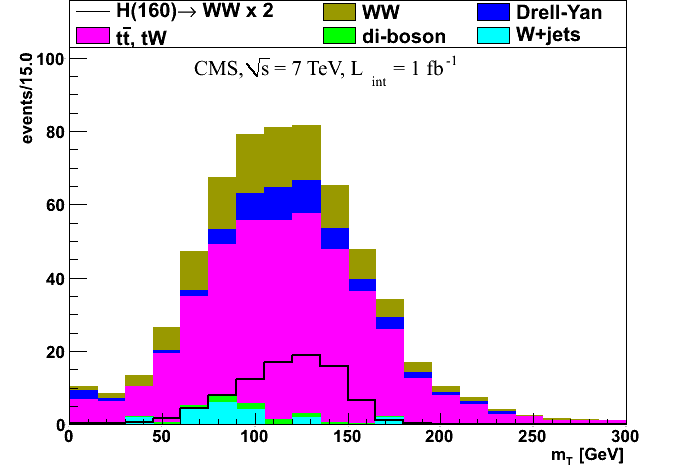
\includegraphics[width=.32\textwidth]{figures/mt_hm160_jets1.png}}
\subfigure[]{
\centering
\label{subfig:mt_hm250_jets1}
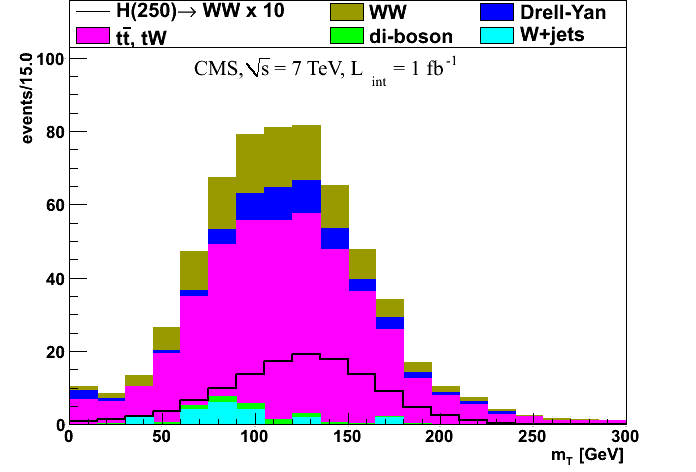
\includegraphics[width=.32\textwidth]{figures/mt_hm250_jets1.png}}\\
\caption{$m_T$ distribution after \WW\ selection for $m_H$=120 $\GeVcc$ \subref{subfig:mt_hm120_jets1}, 
$m_H$=160 $\GeVcc$ \subref{subfig:mt_hm160_jets1} and $m_H$=250 $\GeVcc$ \subref{subfig:mt_hm250_jets1} in the 1-jet bin.}
\label{fig:mt_jets1}
\end{figure}

\begin{figure}[!hbtp]
\centering
\subfigure[]{
\centering
\label{subfig:pmet_hm120_jets1}
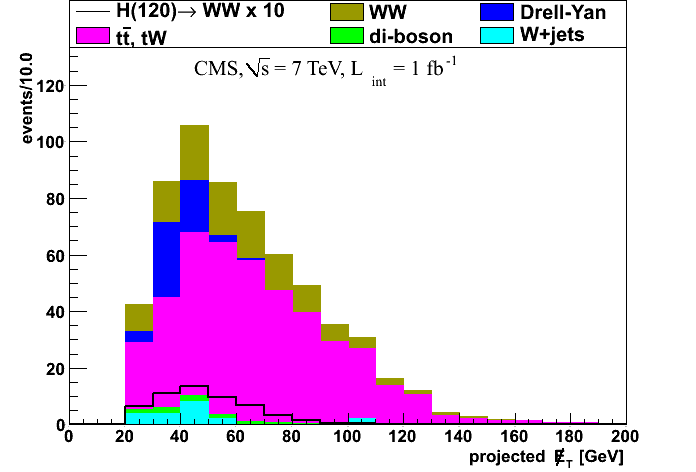
\includegraphics[width=.32\textwidth]{figures/pmet_hm120_jets1.png}}
\subfigure[]{
\centering
\label{subfig:pmet_hm160_jets1}
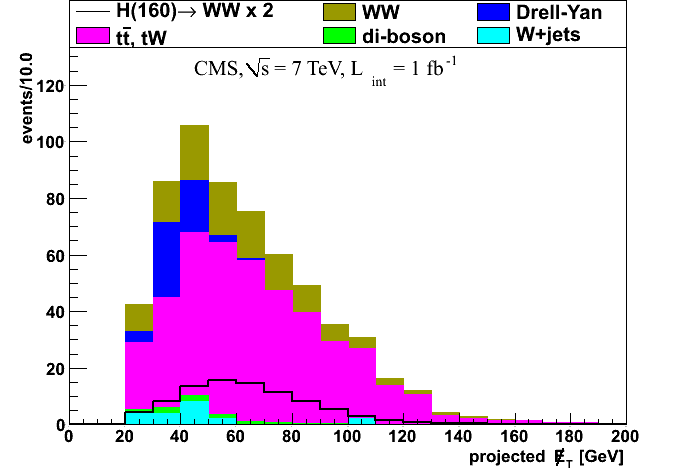
\includegraphics[width=.32\textwidth]{figures/pmet_hm160_jets1.png}}
\subfigure[]{
\centering
\label{subfig:pmet_hm250_jets1}
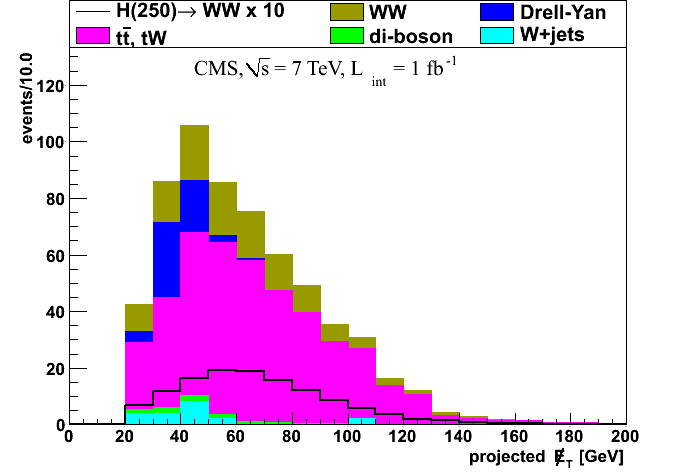
\includegraphics[width=.32\textwidth]{figures/pmet_hm250_jets1.png}}\\
\caption{Projected $\met$ distribution after \WW\ selection for $m_H$=120 $\GeVcc$ \subref{subfig:pmet_hm120_jets1}, 
$m_H$=160 $\GeVcc$ \subref{subfig:pmet_hm160_jets1} and $m_H$=250 $\GeVcc$ \subref{subfig:pmet_hm250_jets1} in the 1-jet bin.}
\label{fig:pmet_jets1}
\end{figure}
